\documentclass[dvipsnames, 9pt]{beamer}

%\documentclass[xcolor=dvipsnames, 8pt]{beamer} %
%\setbeamertemplate{navigation symbols}{}

\usetheme{SantaBarbara}

%light gray/black highlighting to be used with pause command
\colorlet{shadecolor}{gray!40}
\def\blackgray<#1>{%
  \temporal<#1>{\color{shadecolor}}{\color{black}}{\color{shadecolor}}}

\definecolor{black}{HTML}{0A0A0A}
\definecolor{red}{HTML}{e00404} 


\definecolor{blue}{HTML}{0647A8}
\definecolor{darkgreen}{HTML}{008000}

\definecolor{Asparagus}{HTML}{87A96B}

\usepackage[utf8]{inputenc}

\usepackage{tightlist}
\usepackage{tikz, tikzsettings}
\usepackage{verbatim}
\usepackage{amssymb}
\usepackage{amsmath}
\usepackage{amsfonts}
\pdfmapfile{+sansmathaccent.map} % Fix done for making the talk in ubuntu.
\usepackage{algorithmic}
\graphicspath{{./}{./figures/}{./figures/presentation/}}
\usepackage{makecell}
\usepackage{booktabs}

\usepackage{subcaption}
\usepackage[authoryear,round]{natbib}
\usepackage{color}
\usepackage{colortbl}
\usepackage{xcolor}
\usepackage{pgfplots}
\usepackage{ragged2e}
\usepackage{rxn}


\usetikzlibrary{shapes,calc,spy, calc, backgrounds,arrows, fit, decorations.pathmorphing, decorations.pathreplacing, matrix}
\usepackage{caption}
\usepackage{mpcsymbols}
\usepackage{graphicx}

\newcommand{\calert}[1]{\textcolor{blue}{#1}}

\makeatother
\setbeamertemplate{footline}
{\leavevmode%
	\hbox{%
		\begin{beamercolorbox}[wd=.3\paperwidth,ht=2.25ex,dp=1ex,center]{author
		in head/foot}%
			\usebeamerfont{author in head/foot}\insertshortauthor
		\end{beamercolorbox}%
		\begin{beamercolorbox}[wd=.6\paperwidth,ht=2.25ex,dp=1ex,center]{title
		in head/foot}%
			\usebeamerfont{title in head/foot}\insertshorttitle
		\end{beamercolorbox}%
		\begin{beamercolorbox}[wd=.1\paperwidth,ht=2.25ex,dp=1ex,center]{date in
		head/foot}%
			\insertframenumber{} / \inserttotalframenumber\hspace*{1ex}
	\end{beamercolorbox}}%
	\vskip0pt%
}

\renewcommand{\vec}{\textnormal{vec}} 
\newcommand{\stoi}{\text{\boldmath $\nu$}}


\title[Citation informed NODE]{Towards a citation-informed neural ODE \\ or better \\ \textbf{Tell me when can I become tenured!}}

\author[ChE230D---Dake]{Prithvi Dake}
\institute [UCSB]{Department of Chemical
  Engineering\\
    \pgfuseimage{ucsb-logo}}

\date{ChE 230D Project \\
\today}

%\AtBeginSection[]
%{
%  \begin{frame}
%    \frametitle{Outline}
%    \tableofcontents[currentsection]
%  \end{frame}}


\begin{document}

\frame{\titlepage}




\begin{frame}{Outline} 
\tableofcontents
\end{frame}

\section{Compartment model for citation dynamics}
\subsection{Parallels with epidemiological SIR model}
\begin{frame}{Parallels with epidemiological SIR model \small{(citation begets citations)}}
\begin{itemize}
\item Citation dynamics describes the number of references received by the article or other scientific work over time (and numerous studies have been conducted over it)\footnote{\tiny{Reia, S.M. and Fontanari, J.F., 2021. A SIR epidemic model for citation dynamics. The European Physical Journal Plus}}
\item What if we let S = Susceptibles, I = Influencers and R = Recovered/Adopters ?\footnote{\tiny {ZombieTown USA \href{https://mattbierbaum.github.io/zombies-usa}{\textcolor{blue}{Here's the link!}}}}
\end{itemize}
\begin{figure}[H]
\centering
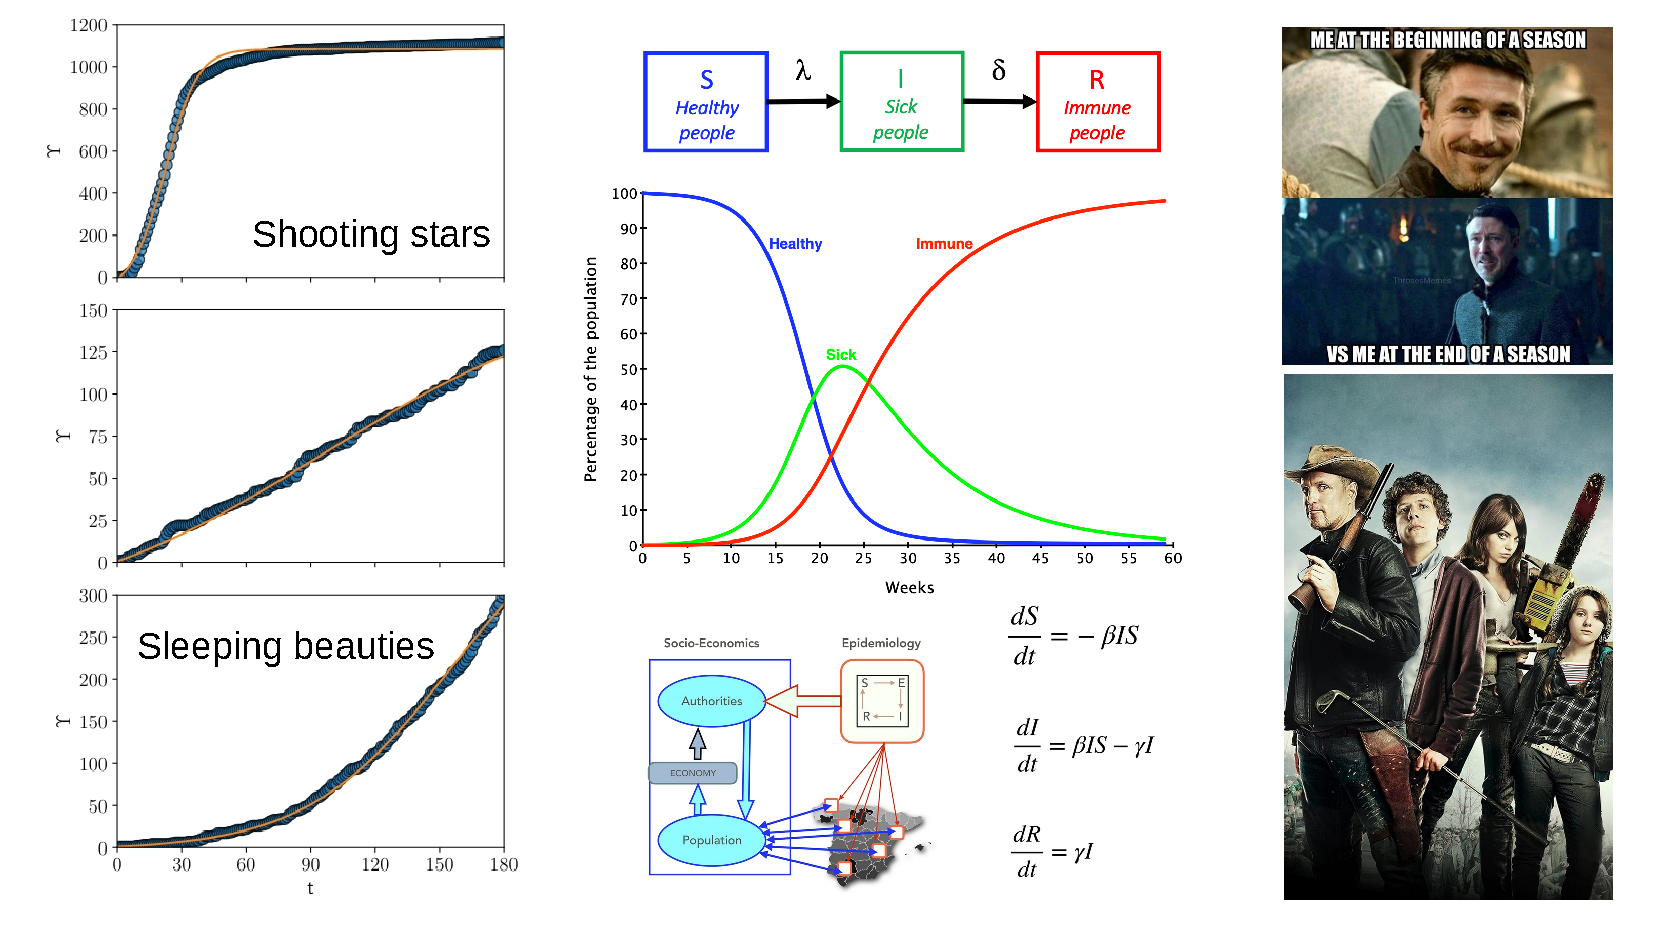
\includegraphics[width=0.85\textwidth]{SIR}
\end{figure}
\end{frame}

\subsection{A$\rightleftharpoons$B$\rightarrow$C but with unknown kinetics}
\begin{frame}{A$\rightleftharpoons$B$\rightarrow$C but with unknown kinetics}
  \begin{block}{}
    \begin{enumerate}
\item Determine a ``structure'' of the dynamic model based 
on cumulative citation history (in this case the variable $R$). This model contains NNs 
to represent the unknown functions that are challenging to parameterize 
and maintain
\begin{align*}
\dfrac{d \mathbf{x}}{d t} &= \mathbf{f}(\mathbf{x, z}; \theta_{NN}) \\
\mathbf{z(t)} &= [\mathbf{x'_{t-1},x'_{t-2} \ldots x'_{t-\Delta}}]'\\
\mathbf{x} \in \R^3 &\qquad \mathbf{f} \in \R^3 \rightarrow \R^3
\end{align*}
\item Similar to S$\rightleftharpoons$I$\rightarrow$R but with unknown kinetics (or rather parameters that depend on many \textit{features})
\item Notice that $I(t_0) = R(t_0) = 0$ while $S(t_0) = S_0$ a theoretical susceptible number of audience for a given paper.
\item Adding to the complexity is the fact that $S$ and $I$ are imaginary intermediates\footnote{\tiny{`imaginary' here means dummy variables, not complex}} that cannot be quantified easily.
\item Conservation law: $S(t_0) = S(t) + I(t) + R(t)$
\item Obviously  true law: $\mathbf{x} \geq 0$
\end{enumerate}
  \end{block}
\end{frame}
\section{Neural ODE framework}
\subsection{Multistep ahead prediction error minimization}
\section{PINNS}
\subsection{How are citation constraints employed in Neural ODE?}
\subsection{Making it smarter}
\section{A limited example}
\section{Resources}

\begin{frame}{Resources}
\begin{figure}[H]
\centering

\includegraphics[width=0.1\textwidth]{jax_logo.png}
\end{figure}
\end{frame}
\end{document}
